\begin{figure}[!htb]
  \centering
  %\begin{subfigure}[b]{0.15\textwidth}
    \begin{tikzpicture}[scale=1.0,auto,swap]

    % the two brain figures on top
    \node (upper_brain) at (0,1.5) { \includegraphics*[scale=\scaleBrainImg,trim=0 0 240 0]{images/dd15Sim2PCA/stage_3.eps}};
    \node (lower_brain) at (0,-1.5) { \includegraphics*[scale=\scaleBrainImg,trim=240 0 0 0]{images/dd15Sim2PCA/stage_3.eps}};
    \node[above=0cm of upper_brain] (stage) {Stage 3};
    % the balls
    
    \end{tikzpicture}
  %\end{subfigure}
  % next subfigure
  \hspace{-1.5em}
  ~
  %\begin{subfigure}[b]{0.15\textwidth}
    \begin{tikzpicture}[scale=1.0,auto,swap]

    % the two brain figures on top
    \node (upper_brain) at (0,1.5) { \includegraphics*[scale=\scaleBrainImg,trim=0 0 240 0]{images/dd15Sim2PCA/stage_6.eps}};
    \node (lower_brain) at (0,-1.5) { \includegraphics*[scale=\scaleBrainImg,trim=240 0 0 0]{images/dd15Sim2PCA/stage_6.eps}};
    \node[above=0cm of upper_brain] (stage) {Stage 6};
    % the balls
    
    \end{tikzpicture}
  %\end{subfigure}
  % next subfigure
  \hspace{-1.5em}
  ~
  %\begin{subfigure}[b]{0.15\textwidth}
    \begin{tikzpicture}[scale=1.0,auto,swap]

    % the two brain figures on top
    \node (upper_brain) at (0,1.5) { \includegraphics*[scale=\scaleBrainImg,trim=0 0 240 0]{images/dd15Sim2PCA/stage_9.eps}};
    \node (lower_brain) at (0,-1.5) { \includegraphics*[scale=\scaleBrainImg,trim=240 0 0 0]{images/dd15Sim2PCA/stage_9.eps}};
    \node[above=0cm of upper_brain] (stage) {Stage 9};
    % the balls
    
    \end{tikzpicture}
  %\end{subfigure}
  % next subfigure
  \hspace{-1.5em}
  ~
  %\begin{subfigure}[b]{0.15\textwidth}
    \begin{tikzpicture}[scale=1.0,auto,swap]

    % the two brain figures on top
    \node (upper_brain) at (0,1.5) { \includegraphics*[scale=\scaleBrainImg,trim=0 0 240 0]{images/dd15Sim2PCA/stage_12.eps}};
    \node (lower_brain) at (0,-1.5) { \includegraphics*[scale=\scaleBrainImg,trim=240 0 0 0]{images/dd15Sim2PCA/stage_12.eps}};
    \node[above=0cm of upper_brain] (stage) {Stage 12};
    % the balls
    
    \end{tikzpicture}
  %\end{subfigure}
  % next subfigure
  \hspace{-1.5em}
  ~
  %\begin{subfigure}[b]{0.15\textwidth}
    \begin{tikzpicture}[scale=1.0,auto,swap]

    % the two brain figures on top
    \node (upper_brain) at (0,1.5) { \includegraphics*[scale=\scaleBrainImg,trim=0 0 240 0]{images/dd15Sim2PCA/stage_15.eps}};
    \node (lower_brain) at (0,-1.5) { \includegraphics*[scale=\scaleBrainImg,trim=240 0 0 0]{images/dd15Sim2PCA/stage_15.eps}};
    \node[above=0cm of upper_brain] (stage) {Stage 15};
    % the balls
    
    \end{tikzpicture}
  %\end{subfigure}
  % next subfigure
  \hspace{-1.5em}
  ~
  \hspace{1em}
  % the red-to-yellow gradient on the right
  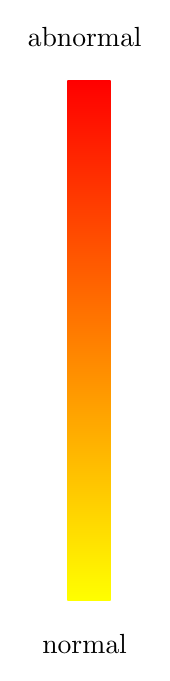
\begin{tikzpicture}[scale=1.1,auto,swap]
    \shade[top color=red,bottom color=yellow] (0,0) rectangle (0.5,6);
    \node[inner sep=0] (corr_text) at (0.2,6.5) {abnormal};
    \node[inner sep=0] (corr_text) at (0.2,-0.5) {normal};
  \end{tikzpicture}
  \caption[Atrophy progression snapshots for PCA subjects using the data-driven EBM]{Atrophy progression snapshots for the PCA subjects using the data-driven EBM. Shown here are several informative stages in the disease progression: 3,6,9,12 and 15. Each brain region is coloured from yellow (normal) to red (abnormal). The positional variance matrix used is the one from sampling method 2 from figure \ref{fig:dd_simultL}. The model suggests that in PCA patients the motor cortex and frontal gyrus are affected first, which is actually not the expected progression of PCA, where posterior regions are usually affected first. However, early motor cortex dysfunction might explain why PCA patients show inability to navigate through space.}
  \label{fig:snap_dd15_sim2_pca}
\end{figure}
